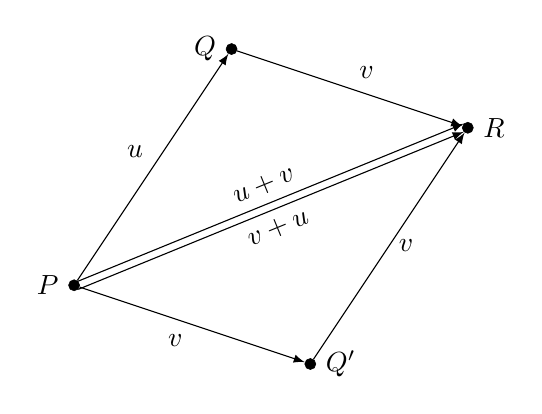
\begin{tikzpicture}[
	point/.style={circle,draw,very thin,fill,inner sep=0pt,minimum size=4pt},
	vector/.style={-latex},
]
	\node[point] at (0,0) (p) [label=left:{$P$}] {};
	\node[point] at (2,3) (q) [label=left:{$Q$}] {};
	\node[point] at (3,-1) (q2) [label=right:{$Q'$}] {};
	\node[point] at (5,2) (r) [label=right:{$R$}] {};
	\draw[vector] (p) to node[above left] {$\uvec{u}$} (q);
	\draw[vector] (p) to node[below left] {$\uvec{v}$} (q2);
	\draw[vector] (q) to node[above right] {$\uvec{v}$} (r);
	\draw[vector] (q2) to node[right] {$\uvec{v}$} (r);
	\draw[vector] (p.north east) to node[above,sloped] {$\uvec{u}+\uvec{v}$} (r.north west);
	\draw[vector] (p.south east) to node[below,sloped] {$\uvec{v}+\uvec{u}$} (r.south west);
\end{tikzpicture}
